\scanpage{30}
\(Z\) est un diviseur sur \(X\times T\) et \(\nu\) sur \(T\) est de degré 0 et tel que \(S_T(\nu)=0\), alors \(Z(\nu)\) est lin. équi. à 0. Or \(\unsure{\operatorname{cl}}Z(\nu)=u(S_T(\nu))\), où \(u:\deleted{\unsure{\operatorname{Alb}}}\ A_T\longrightarrow\underline{\operatorname{Pic}}_X^0\) est l'hom défini pr \(Z\).

\uline{Théorème} 1.\deleted{\unsure{5}}\inserted{6}. Soient \(z,z'\) deux classes dans \(A'{}^*(X)\) alg. équiv. à 0, \(X\) étant \deleted{[projective]}\inserted{\unsure{qu. pr.}}. Alors \(zz'=0\). \inserted{[Si \(X\) est projective, alors il suffit que l'un des facteurs \(z\) soit alg. équiv. à 0, et l'autre \uline{num.} équiv. à 0??]}
\margin{\deleted{À voir si \unsure{il ne suffit pas} \unsure{que pour} \(z\) ou \(z'\) on \unsure{sait} que \unsure{\(\tau\)-équiv.|\(\simeq\)-équiv.} à 0, voire si \(X\) \unsure{n'est pas} \unsure{linéaire|qu. pr.}}}
\margin{\figure{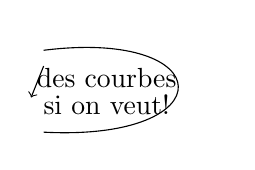
\begin{tikzpicture}[scale=.8]
\node at (0,0) {\shortstack{\unsure{des courbes}\\si on veut!}};
\draw (-1,.65) .. controls (1.8,1) and (1.9,-.8) .. (-1,-.65);
\draw[->] (-1,.4)--(-1.2,-.1);
\end{tikzpicture}}}

\deleted{\unsure{Cela}} \inserted{La première assertion} résulte formellement de la définition de ``alg. équiv. à 0'' \inserted{(via variétés \(T\) \uline{projectives} \uline{lisses} connexes)} et du fait que si \(T,T'\) sont deux \inserted{telles} variétés, \deleted{et} (leur connexité suffit) et \(x,y\) sont deux points de \(T\), \(x'\) et \(y'\) deux pts de \(T'\), alors
\[
\nu=\inserted{((x)-(y))\times((x')-(y'))=}(x,x')-(x,y')-(y,x')+(y,y')
\]
est tel que \(\deleted{\unsure{\nu\in A}}\ S_{T\times T'}(\nu)=0\).
\margin{NB. On ignore si cet \(\nu\) est \uline{lin.} équiv. à 0, $=$ si \(T,T'\) sont des \uline{courbes}!}

[Il y a intérêt à transformer \deleted{le Pb} \inserted{l'énoncé} en un énoncé sur l'opération \(\times\).]
\mspage{29}
